\section{eplusout.eso}

The standard output file from EnergyPlus. It includes all the applicable variables selected with the “Output:Variable” commands as well as those with the “Output:Meter” commands. All levels of frequency of reporting are included intermingled as occurs in the running of the program. The form of the file is a data dictionary, followed by the data.

In this case, the dictionary portion of the file comes first followed by an “end of data dictionary line” and then the data makes up the rest of the file.

Thus, the basic structure of the standard output file is:

\begin{lstlisting}
Data Dictionary Information
End of Data Dictionary
Data
...
Data
End of Data
\end{lstlisting}

As with the IDF structure, there are rules associated with the interpretation of the standard output data dictionary. These rules are summarized as follows:

\begin{itemize}
  \item The first item on each line is an integer which represents the “report code”. This “report code” will be listed in the data section where it will also be the first item on each line, identifying the data. Only 2 lines in the output file will not have an integer as the first item (“End of Data Dictionary” and “End of Data” lines).

  \item The second item on each line is also an integer. This integer corresponds to the number of items left on the dictionary line. Each string consists of a variable name and units in square brackets. Square brackets are required for all strings. If there are no units associated with a particular variable, then there are no characters between the brackets.
\end{itemize}

Six standard items appear at the start of every EnergyPlus Standard Output File Data Dictionary:

\begin{lstlisting}
Program Version,EnergyPlus <version number indicated>
  1,5,Environment Title[],Latitude[deg],Longitude[deg],Time Zone[],Elevation[m]
  2,6,Day of Simulation[],Month[],Day of Month[],DST Indicator[1 = yes 0 = no],Hour[],StartMinute[],EndMinute[],DayType
  3,3,Cumulative Day of Simulation[],Month[],Day of Month[],DST Indicator[1 = yes 0 = no],DayType  ! When Daily Report Variables Requested
  4,2,Cumulative Days of Simulation[],Month[]  ! When Monthly Report Variables Requested
  5,1,Cumulative Days of Simulation[] ! When Run Period Report Variables Requested
\end{lstlisting}

Item 0 is the program version statement.

Item 1 is produced at the beginning of each new “environment” (design day, run period).

Item 2 is produced prior to any variable reported at the timestep or hourly intervals. Hourly intervals will be shown with a start minute of 0.0 and an end minute of 60.0. Timestep intervals will show the appropriate start and end minutes.

Item 3 is produced prior to any variable reported at the daily interval.

Item 4 is produced prior to any variable reported at the monthly interval.

Item 5 is produced prior to any variable reported at the end of the “environment”.

Following these five standard lines will be the variables requested for reporting from the input file (ref. Report Variable). For example:

\begin{lstlisting}
6,2,Environment,Site Outdoor Air Drybulb Temperature [C] !Hourly
21,2,ZONE ONE,Zone Mean Air Temperature [C] !Hourly
22,2,ZONE ONE,Zone Total Latent Gain [J] !Hourly
26,2,ZONE ONE,Zone Lights Electric Energy [J] !Hourly
\end{lstlisting}

This example illustrates the non-consecutive nature of the “report codes”. Internally, EnergyPlus counts each variable that *could* be reported. This is the assigned “report code”. However, the user may not request each possible variable for reporting. Note that, currently, the requested reporting frequency is shown as a comment (!) line in the standard output file.

The data is produced when the actual simulation is performed (after the warmup days unless the Output:Diagnostics requesting ReportDuringWarmup is used). Data output is simpler in format than the data dictionary lines. From the dictionary above:

\begin{lstlisting}
     1,DENVER COLORADO WINTER,  39.75,-104.87,  -7.00,1610.26
     2,  1, 1,21, 0, 1, 0.00,60.00,Monday
6,-17.22222
21,-17.22219
22,0.0000000E+00
26,0.0000000E+00
     2,  1, 1,21, 0, 2, 0.00,60.00,Monday
6,-17.22222
21,-17.22219
22,0.0000000E+00
26,0.0000000E+00
     2,  1, 1,21, 0, 3, 0.00,60.00,Monday
6,-17.22222
21,-17.22219
22,0.0000000E+00
26,0.0000000E+00
…
\end{lstlisting}

This output file can be easily turned into a form that is read into commonly used spreadsheet programs where it can be further analyzed, graphed, etc.

\begin{figure}[hbtp] % fig 4
\centering
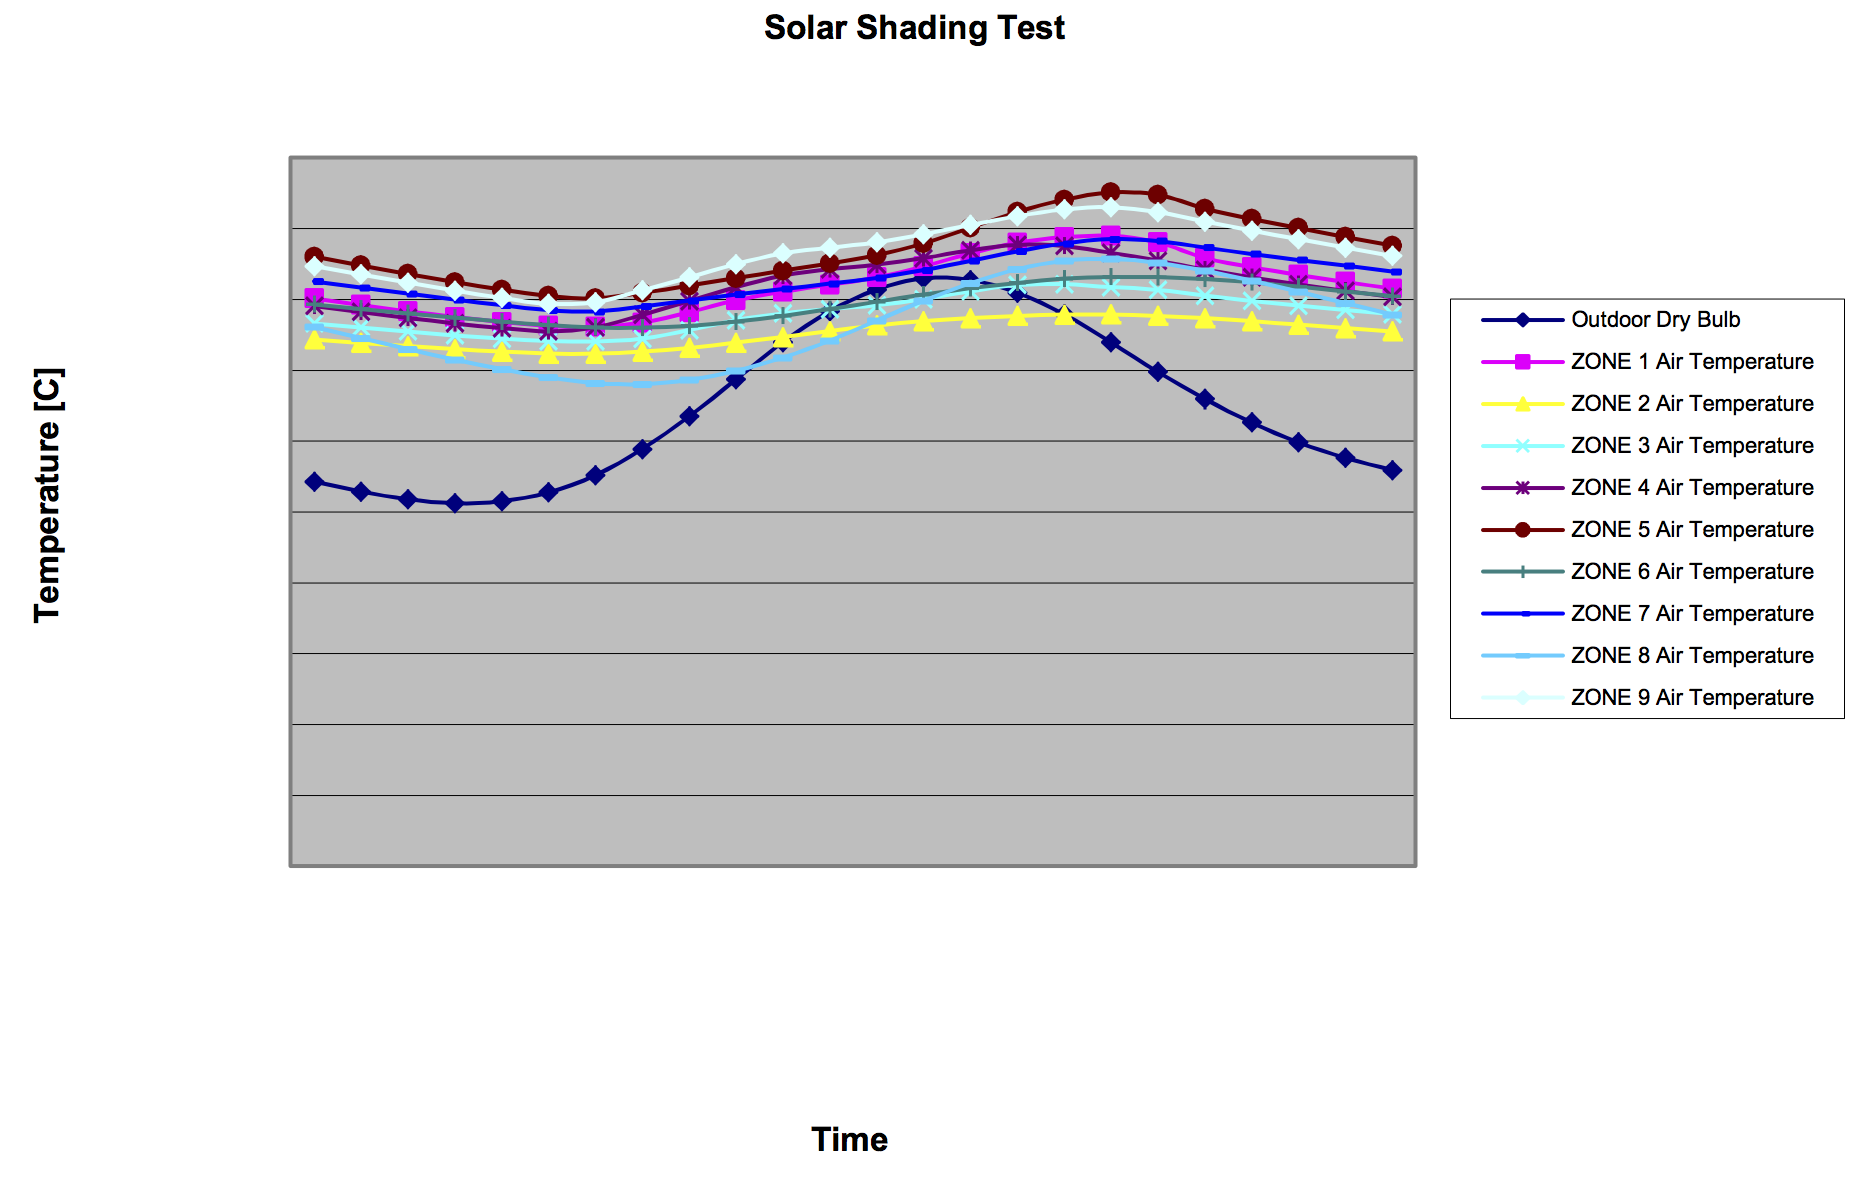
\includegraphics[width=0.9\textwidth, height=0.9\textheight, keepaspectratio=true]{media/image014.png}
\caption{Example Chart from Standard Output File \label{fig:example-chart-from-standard-output-file}}
\end{figure}

\begin{lstlisting}
Program Version,EnergyPlus, <version>
     1,5,Environment Title[],Latitude[deg],Longitude[deg],Time Zone[],Elevation[m]
     2,6,Day of Simulation[],Month[],Day of Month[],DST Indicator[1 = yes 0 = no],Hour[],StartMinute[],EndMinute[],DayType
     3,3,Cumulative Day of Simulation[],Month[],Day of Month[],DST Indicator[1 = yes 0 = no],DayType  ! When Daily Report Variables Requested
     4,2,Cumulative Days of Simulation[],Month[]  ! When Monthly Report Variables Requested
     5,1,Cumulative Days of Simulation[] ! When Run Period Report Variables Requested
6,2,Environment, Site Outdoor Air Drybulb Temperature [C] !Hourly
429,2,RESISTIVE ZONE, Zone Air System Sensible Heating Energy [J] !Hourly
450,2,RESISTIVE ZONE, Zone Air System Sensible Cooling Energy [J] !Hourly
458,2,RESISTIVE ZONE, Zone Air Temperature [C] !Hourly
463,2,EAST ZONE, Zone Air System Sensible Heating Energy [J] !Hourly
469,2,EAST ZONE, Zone Air System Sensible Cooling Energy [J] !Hourly
472,2,EAST ZONE, Zone Air Temperature [C] !Hourly
477,2,NORTH ZONE, Zone Air System Sensible Heating Energy [J] !Hourly
483,2,NORTH ZONE, Zone Air System Sensible Cooling Energy [J] !Hourly
486,2,NORTH ZONE, Zone Air Temperature [C] !Hourly
491,2,SimHVAC, HVAC System Solver Iteration Count !Hourly
521,2,SimAir, Air System Simulation Maximum Iteration Count !Hourly
<reduced for brevity>
\end{lstlisting}

\begin{lstlisting}
End of Data Dictionary
  1,CHANUTE AFB ILLINOIS SUMMER,  40.30, -88.13,  -6.00, 229.51
  2,   1, 7,21, 0, 1, 0.00,60.00,Monday
6,21.2884261500000
429,0.000000000000000E+000
450,0.000000000000000E+000
458,31.1054947436037
463,0.000000000000000E+000
469,0.000000000000000E+000
472,31.2222148107451
477,0.000000000000000E+000
483,0.000000000000000E+000
486,31.5855358697037
\end{lstlisting}

Each report variable (ref: eplusout.rdd) is assigned an identification number, as in the line:

\begin{lstlisting}
486,2,NORTH ZONE,Zone Air Temperature [C] !Hourly
\end{lstlisting}

\textbf{\#486} is the id number of the Zone/Sys Air Temperature value for the North Zone.

\textbf{2} – is the number of parameters on the line

\textbf{North Zone} – the identifying “key name” for the line

\textbf{Zone Air Temperature [C]} – the actual report variable name along with units [C]

\textbf{! Hourly} – the ! is the standard comment character, information following this character reminds the user how frequently this data will appear in the following.

As another example:

Each \textbf{Output:Variable} object causes a specific number assignment for outputs. For example, you could request separate reporting for the outside temperature:

\begin{lstlisting}
Output:Variable,*, Site Outdoor Air Drybulb Temperature,timestep;
Output:Variable,*, Site Outdoor Air Drybulb Temperature,hourly;
Output:Variable,*, Site Outdoor Air Drybulb Temperature,monthly;
\end{lstlisting}

And the following would appear in the standard output file:

\begin{lstlisting}
6,2,Environment,Site Outdoor Air Drybulb Temperature [C] !TimeStep
7,2,Environment,Site Outdoor Air Drybulb Temperature [C] !Hourly
8,2,Environment,Site Outdoor Air Drybulb Temperature [C] !Monthly [Value,Min,Day,Hour,Minute,Max,Day,Hour,Minute]
\end{lstlisting}

Item \# 6 will be listed following the TimeStep timestamp for each timestep. Item \#7 will be listed following an hourly timestamp. And item \#8 will be listed following a monthly timestamp and has additional fields (because it is an “average” variable) that show the minimum and maximum values with identifying times for those minimum and maximum. An excerpt will illustrate:

\begin{lstlisting}
     2,  1, 7,21, 0, 1, 0.00,15.00,Monday** – timestep timestamp**
6,17.08889
48,21.39851
49,0.0000000E+00
53,0.0000000E+00
60,21.87214
     2,  1, 7,21, 0, 1, 0.00,60.00,Monday** – hourly timestamp**
7,16.75555
     4,  1, 7** – monthly timestamp**
8,22.77037,15.00000,21, 4,60,32.77778,21,14,60
\end{lstlisting}

To interpret, the first value (\#6) is 17.09 C, \#7 is 16.76 C (average for the hour), and \#8 is 22.77 C, the average for the month with the low (minimum) of 15 C occurring on 7/21 4:60 (or 5:00) and the high (maximum) occurring on 7/21 14:60 (or 15:00).
